%!TEX root = ../template.tex
%%%%%%%%%%%%%%%%%%%%%%%%%%%%%%%%%%%%%%%%%%%%%%%%%%%%%%%%%%%%%%%%%%%%
%% chapter6.tex
%% NOVA thesis document file
%%
%% Chapter with the vision system description.
%%%%%%%%%%%%%%%%%%%%%%%%%%%%%%%%%%%%%%%%%%%%%%%%%%%%%%%%%%%%%%%%%%%%
\chapter{Vision System}
\label{cha:vision_system}

\begin{quotation}
\begin{flushright}
\itshape
«Quotation»\\
\textbf{- Author}
\end{flushright}
\end{quotation}

The vision system is a vital component of the whole system's architecture. On this chapter, a detailed description of this system will be provided. The chapter will start with a general system overview. It will follow with a physical description of the camera, the camera operation, then the camera attachment to the robot, and later, camera calibration. The chapter will end with an overview of the integrations with \gls{ros} and Gazebo.

% ==========================
% = Overview =
% ==========================

\section{Overview}
\label{sec:vision_system_overview}

The vision system is composed by an Intel\textregistered RealSense\texttrademark{} D415 depth camera. It provides not only \gls{rgb} data but also \glsfirst{ir} and depth data.\\

The camera is small, lightweight, low cost, and it is suitable for indoor or outdoor environments. It has high resolution in both \gls{rgb} and depth data, and up to 90 \gls{fps} of frame rate for depth data. It features a range from 0.16 to 10 \si{\meter}.

It has self-calibration capabilities controlled via its open source \gls{sdk}. The \gls{sdk} has wrappers for several languages and platforms, including \gls{ros}.

% section vision_system_overview

% ==========================
% = Physical Description =
% ==========================

\section{Physical Description}
\label{sec:vision_system_physical_description}

D415 depth camera has a small form factor of $29 \times 20 \times 23$ \si{\milli\meter} (Length $\times$ Depth $\times$ Height). Inside, it has an Intel\textregistered{} RealSense\texttrademark{} Vision Processor D4 and a Depth Module. The vision processor is common among the D400 camera series. The depth module for this camera features an \gls{ir} projector, two imagers (left and right) for stereo vision, and an \gls{rgb} camera (Fig. \ref{fig:camera_physical_description}).\\

The camera has USB-C connector and comes with a USB-C/USB-A cable to connect the camera to a computer. It comes with 3 mounting points, two M3 thread holes on the back of the camera, and one 1/4‑20 UNC thread mounting point on the bottom, not visible on Figure \ref{fig:camera_physical_description}. A tripod stand is also supplied to be assembled on the 1/4-20 UNC mounting point. It also features an external sensor sync connector on the top side.

The most important technical specifications are presented on table \ref{tab:camera_tech_specs}.\\

\begin{figure}[htbp]
	\centering
	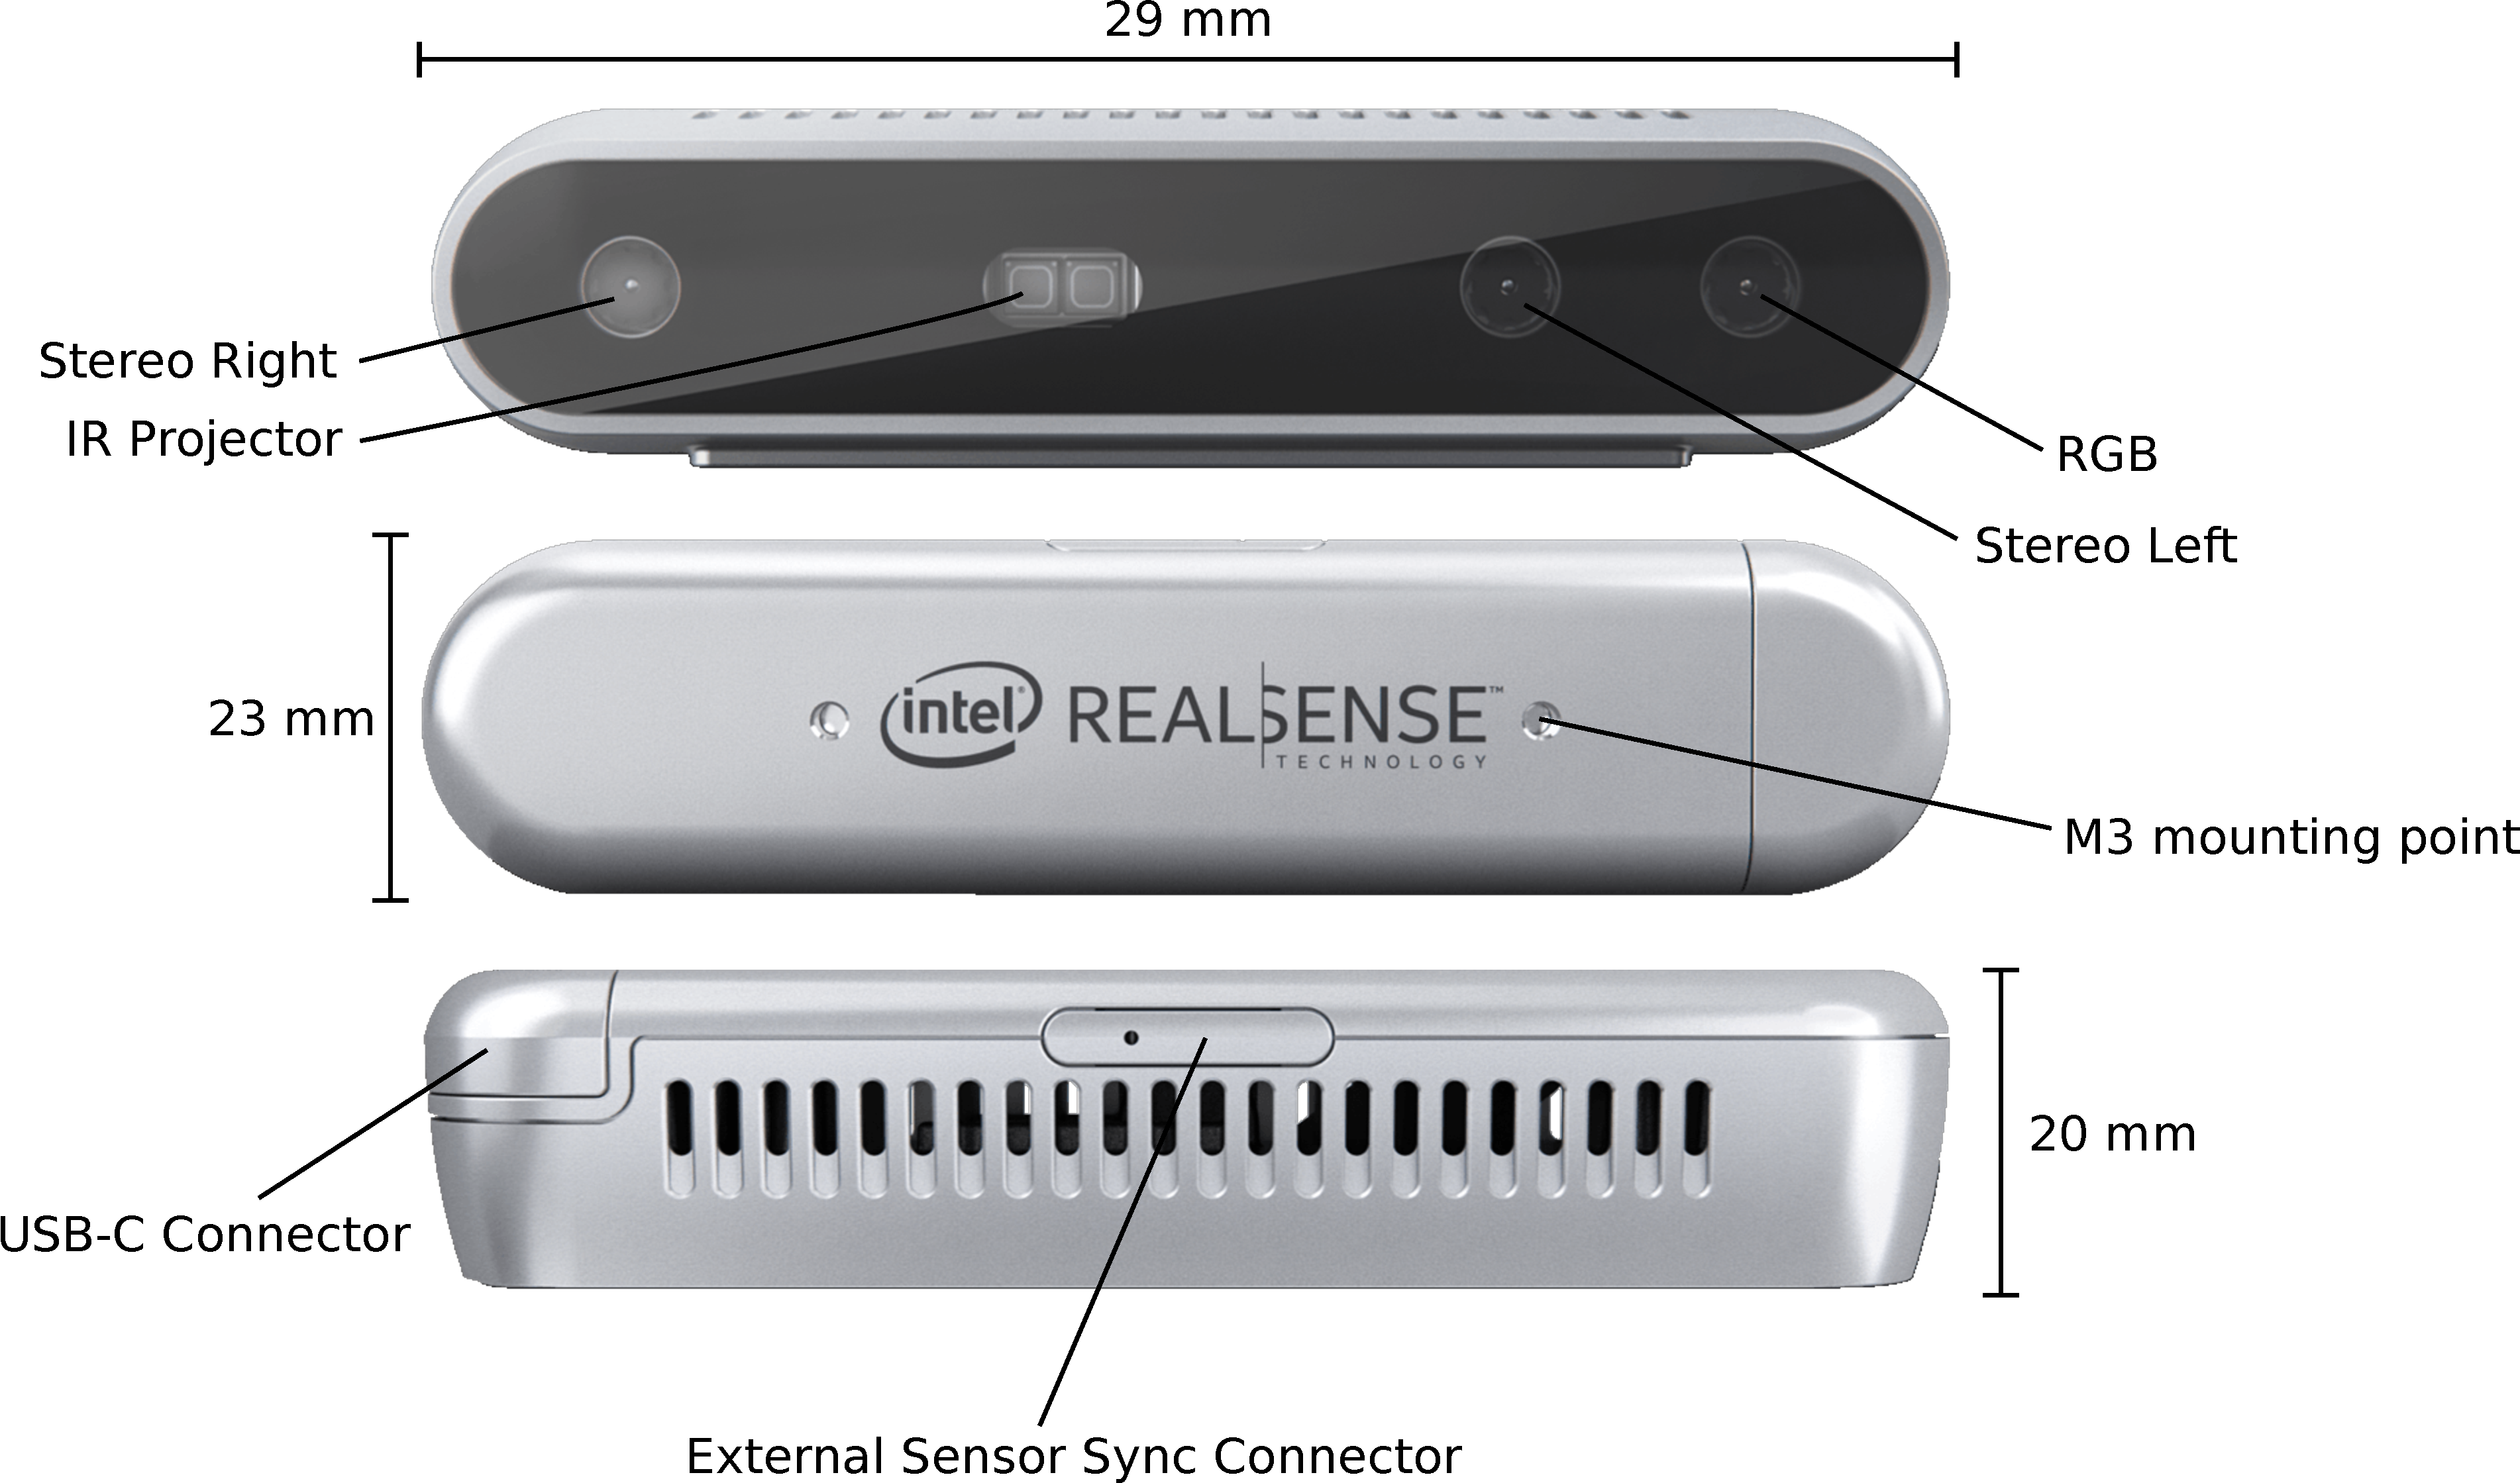
\includegraphics[width=\textwidth]{camera_physical_description}
	\caption{Intel\textregistered{} RealSense\texttrademark{} D415 camera's physical description. Courtesy of Intel\textregistered{} and adapted from \cite{IntelRealSense_depth_camera_d415}.}
	\label{fig:camera_physical_description}
\end{figure}

More detailed technical information about the camera is available on the camera datasheet which is partially available as annex \ref{ann:d415_datasheet}.

\begin{table}[htbp]
    \caption{Intel\textregistered{} RealSense\texttrademark{} D415 camera technical specifications. Courtesy of Intel\textregistered{} and adapted from \cite{IntelRealSense_depth_camera_d415}.}
    \centering
    \resizebox{\textwidth}{!}{%
    \begin{tabular}{c|l|l}
    \toprule
         \multirow{5}{*}{\textbf{Features}} & \textbf{Use Environment:} & \textbf{Maximum Range:} \\
            & Indoor/Outdoor & Approx. 10 meters. Accuracy varies \\
            & \textbf{Image Sensor Technology:} & depending on calibration, scene, \\
            & Rolling Shutter, 1.4\si{\micro\meter} × 1.4\si{\micro\meter} & and lighting condition. \\
            & pixel size & \\
    \midrule
         \multirow{6}{*}{\textbf{Depth}} & \textbf{Depth Technology:} & \textbf{Depth Field of View (FOV):}\\
         & Active IR Stereo & $65°\pm2° × 40°\pm1° × 72°\pm2°$ \\
         & \textbf{Minimum Depth Distance (Min-Z):} & \textbf{Depth Output Resolution:} \\
         & 0.16 m & Up to 1280 × 720 \\
         & & \textbf{Depth Frame Rate:} \\
         & & Up to 90 fps \\
    \midrule
         \multirow{4}{*}{\textbf{RGB}} & \textbf{RGB Sensor Resolution:} & \textbf{RGB Sensor FOV (H × V × D):} \\
         & 1920 × 1080 & 69.4° × 42.5° × 77° (±3°) \\
         & \textbf{RGB Frame Rate:} & \\
         & 30 fps & \\
    \midrule
         \textbf{Major} &  \textbf{Camera Module:} & \textbf{Vision Processor Board:} \\
         \textbf{Components} & Intel RealSense Module D415 & Intel RealSense Vision Processor D4 \\
    \midrule
         \multirow{5}{*}{\textbf{Physical}} & \textbf{Form Factor}: & \textbf{Connectors:} \\
         & Camera Peripheral & USB‑C* 3.1 Gen 1* \\
         & \textbf{Length × Depth × Height:} & \textbf{Mounting Mechanism:} \\
         & 99 mm × 20 mm × 23 mm & – One 1/4‑20 UNC thread mounting point.\\
         & & – Two M3 thread mounting points. \\
    \bottomrule
    \end{tabular}}
    \label{tab:camera_tech_specs}
\end{table}

% section vision_system_physical_description

% ==========================
% = Camera Operation =
% ==========================

\section{Camera Operation}
\label{sec:vision_system_camera_operation}

On this section, the camera operation will be briefly explained. The camera's depth data is obtained through a stereo vision mechanism. The stereo vision system consists of two imagers, left and right, and an \gls{ir} projector. 

The \gls{ir} projector is only needed in scenes with low texture to improve depth accuracy. It accomplishes this improvement by projecting a static IR pattern (Fig. \ref{fig:camera_stereo_vision_mechanism}).

The role of the imagers is to capture the scene and send it to the depth imaging (vision) processor. This processor is responsible for generating the depth data "by correlating points on the left image to the right image and via shift between a point on the Left image and the Right image" \cite{} {\color{red} falta citar! tem que ser manualmente. usar tipo @manual} (Fig. \ref{fig:camera_stereo_vision_mechanism}). The set of data for all the pixels forms a depth frame, and a set of depth frames forms a depth video stream.\\

A clarification must be done on the concept of depth. There is a difference between depth and range. Range is the linear distance between the observed object and the camera. Depth, is the perpendicular distance between the object and the camera's lens plane (Fig. \ref{fig:camera_depth_vs_range}). The depth distance is less than or equal to the range.

\begin{figure}[htbp]
	\centering
	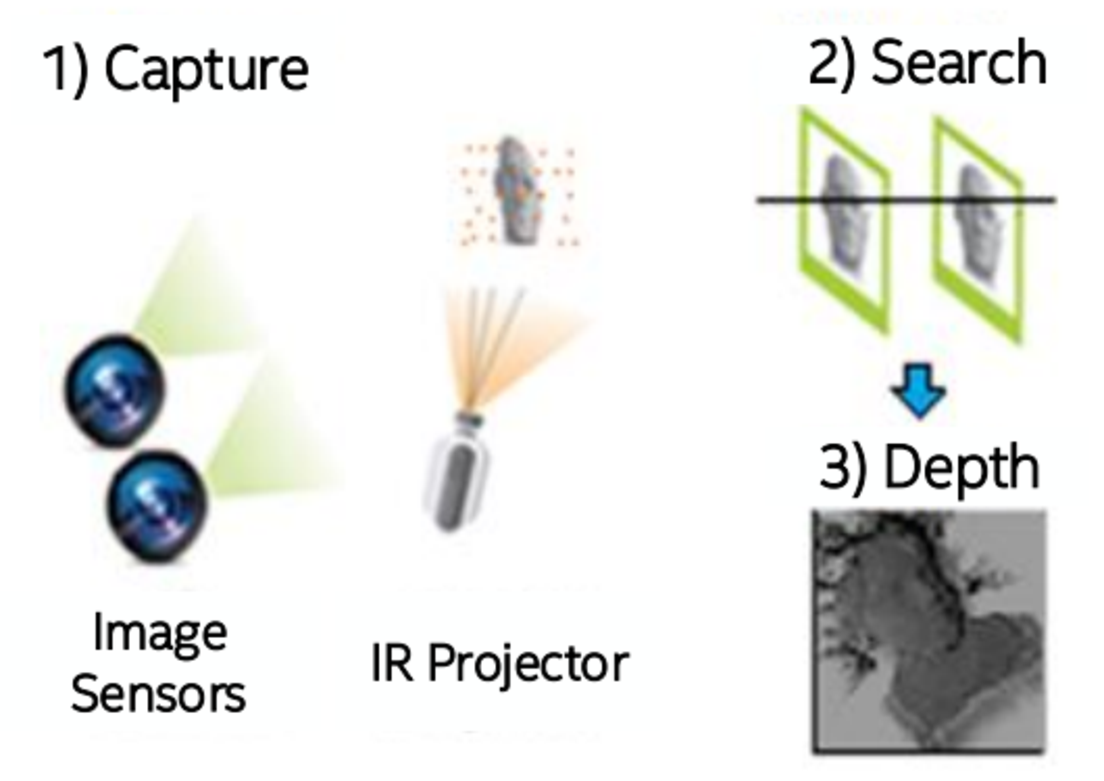
\includegraphics[width=0.7\textwidth]{camera_stereo_vision_mechanism}
	\caption{Camera Stero Vision Technology. (1) Left and Right imagers capture the scene while the \gls{ir} projects a static pattern. (2) The images from both imagers are correlated pixel by pixel and their shifts calculated. (3) Depth data is obtained from these correlated shifts.}  
	\label{fig:camera_stereo_vision_mechanism}
\end{figure}

\begin{figure}[htbp]
	\centering
	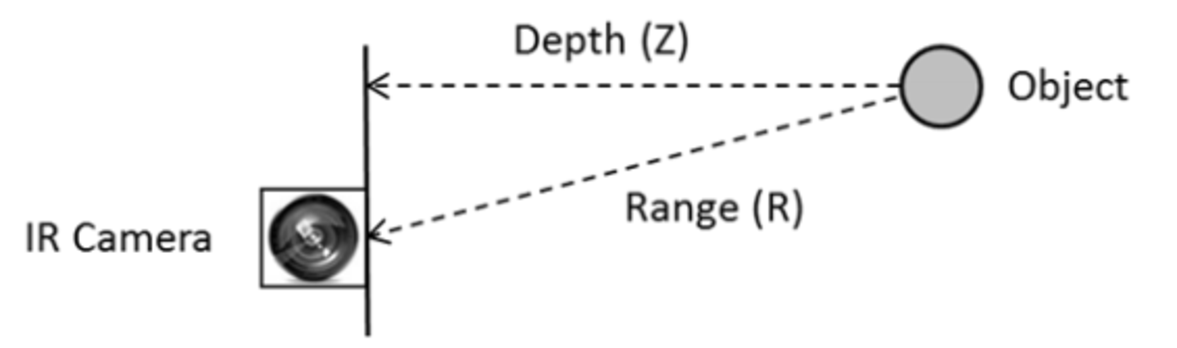
\includegraphics[width=.7\textwidth]{camera_depth_vs_range}
	\caption{Difference between Depth and Range. Range is the linear distance from the object to the camera. Depth is the perpendicular distance between the object and the camera's lens plane.}
	\label{fig:camera_depth_vs_range}
\end{figure}

% section vision_system_camera_operation

% ==========================
% = Camera Attachment to Robot =
% ==========================

\section{Camera Attachment to Robot}
\label{sec:vision_system_camera_attachment}

The way the system was projected established a camera-robot relationship of the type eye-in-hand, which means the camera is attached to the robot. This section will describe the attachment mechanism and location of the camera on the robot.\\

Because the goal of the camera was to assess the patient wounds, it was important for the camera to be place close to, or directly on the end-effector. By placing at that position the camera \gls{fov} could be adjusted by robot movement to optimise the wound assessment.

The choice was to attach it to the Pilot, on an existent groove above the Pilot's Grip (Fig. \ref{fig:camera_attachment_site}). This particular placement allows the camera to see the area in front of the end-effector.

\begin{figure}[htbp]
	\centering
	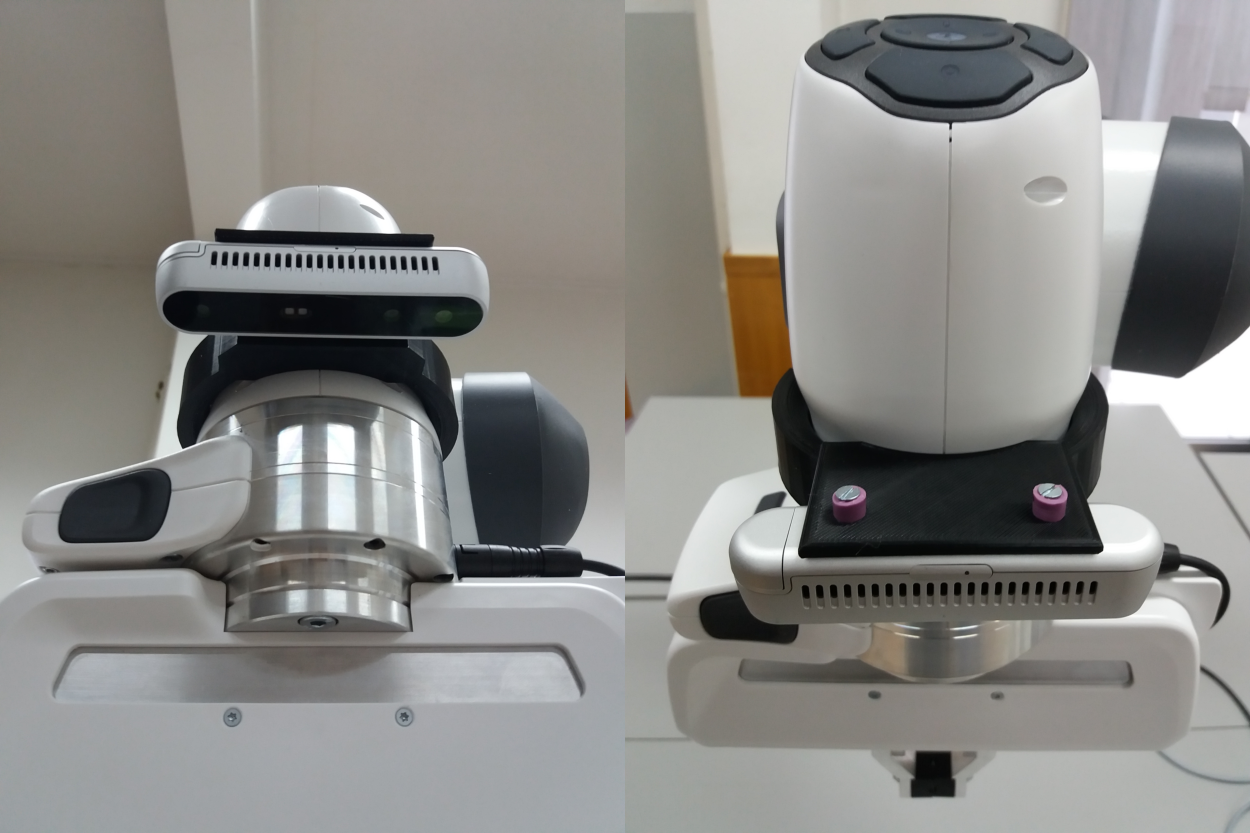
\includegraphics[width=.8\textwidth]{camera_attachment_site}
	\caption{Camera attachment site on the robotic arm. The camera holder is attached to the Pilot's groove above the Grip. The fixation mechanism is by compression force. The camera is fixed on the holder by two M3 thread screws.}
	\label{fig:camera_attachment_site}
\end{figure}

\subsection{Camera Holder}
\label{subsec:vision_system_camera_attachment_holder}

In order to attach the camera to the robot a custom-made holder was designed using \gls{cad} tools and 3D printed in PLA thermoplastic. 

The goal of the design was for the holder to embrace the Pilot's groove and stay fixed only through compression forces. This way the camera is statically fixed but has some leeway to adjust its orientation. The holder used the M3 mounting points to secure the camera, because M3 thread screws are more easily available than 1/4‑20 UNC thread screws.

Figure \ref{fig:camera_holder_render} shows a 3D model render of the camera holder. For mechanical specifications consult appendix \ref{app:camera_holder_mechanical_drawings}.

\begin{figure}[htbp]
	\centering
	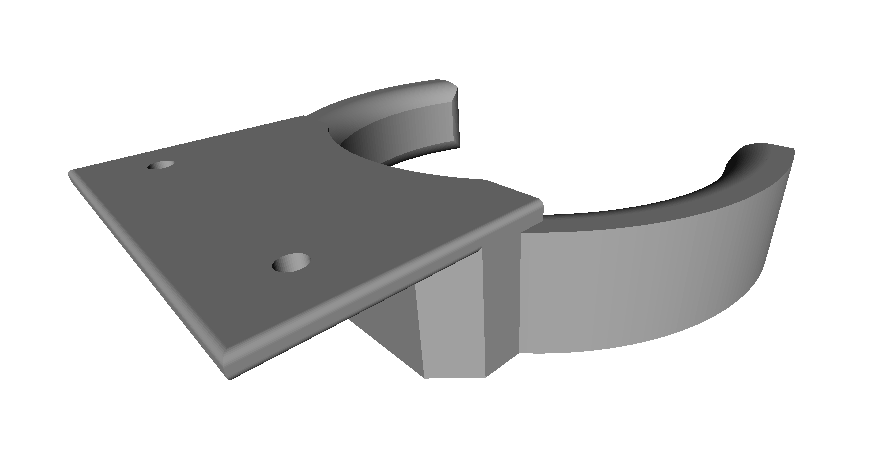
\includegraphics[width=\textwidth]{camera_holder_render}
	\caption{Camera holder 3D model render.}
	\label{fig:camera_holder_render}
\end{figure}

% section vision_system_camera_attachment

% ==========================
% = Camera Calibration =
% ==========================

\section{Camera Calibration}
\label{sec:vision_system_camera_calibration}

Whenever there is a system composed by a robot and a camera that work together, a calibration must be done. In general, the calibration serves to obtain the camera \textit{intrinsic} and \textit{extrinsic} parameters. The intrinsic parameters are related to the camera optical system, while the extrinsic parameters are related to the camera coordinates in relation to a reference frame.

In this thesis, the intrinsic parameters are not calculated because the camera has self-calibration capabilities. However, the extrinsic parameters are needed. They allow the calculation of the transformation matrix, $\boldsymbol{H}^b_c$, between the camera frame and robot base frame.

Without this calibration, an approximation of the transformation matrix can be obtained in \gls{ros}. By defining the approximate position of the joint between the camera model and robot model, \textbf{tf} package can provide a transformation matrix.

\subsection{Calibration Procedure}
\label{subsec:vision_system_camera_calibration_procedure}

% subsection vision_system_camera_calibration_procedure

\subsection{Calibration Results}
\label{subsec:vision_system_camera_calibration_results}

% subsection vision_system_camera_calibration_results

% section vision_system_camera_calibration

% ==========================
% = Integration with ROS =
% ==========================

\section{Integration with ROS}
\label{sec:vision_system_integration_ros}

As said earlier, the D415 depth camera comes with an \gls{sdk} wrapper for \gls{ros}. The \gls{sdk} supplies several important tools for development. One such tool is an application, Intel\textregistered{} RealSense\texttrademark{} Viewer, that can be used to view, record and playback data streams. It also allows the user to set configurations and even update the camera's firmware.

The \gls{ros} wrapper has two packages, \textit{realsense2\_camera} and \textit{realsense2\_description}. The former is responsible for handling the data streams and making them available through \gls{ros} topics. The latter defines the camera model for visualisation.

On appendix \ref{app:ros_setup}, section \ref{sec:ros_setup_camera}, all the setup details are provided for the integration with \gls{ros}.

% section vision_system_integration_ros

% ==========================
% = Integration with Gazebo =
% ==========================

\section{Integration with Gazebo}
\label{sec:vision_system_integration_gazebo}

In order to use the camera on the simulated environment, a specific configuration must be done. The models provided on \textit{realsense2\_description} can be used to visualise the camera on Gazebo, but they cannot provide data. For that, a few changes must be done to create a Gazebo camera plugin to simulate all three data streams, \gls{rgb}, \gls{ir} and depth. The description files also need to be updated to attach the camera on the robot at the right place.

All the changes needed to properly simulate the camera are addressed on appendix \ref{app:gazebo_setup}, section \ref{sec:vision_system_integration_gazebo}.

% section vision_system_integration_gazebo